\chapter{Проверки}\label{ch:proverki}

\textbf{Что вы узнете:} что ловит кнопка «Проверить», как читать список замечаний и как их исправлять.

\section{Что проверяет симулятор}

Кнопка \knopka{Проверить} запускает шоу в симуляции, а список появляется на вкладке \knopka{Проверки}. Каждая строка бывает одного из трёх уровней.
\begin{itemize}
  \item \textbf{Ошибка}: так лететь нельзя. Кнопка \knopka{Загрузить} недоступна.
  \item \textbf{Замечание} (предупреждение): лететь можно, но стоит подумать.
  \item \textbf{Сведение}: просто полезная информация.
\end{itemize}
Наверху списка видны числа: «ошибок 0, замечаний 1, сведений 1». Ошибки всегда идут первыми.

\begin{figure}[H]
  \centering
  \fbox{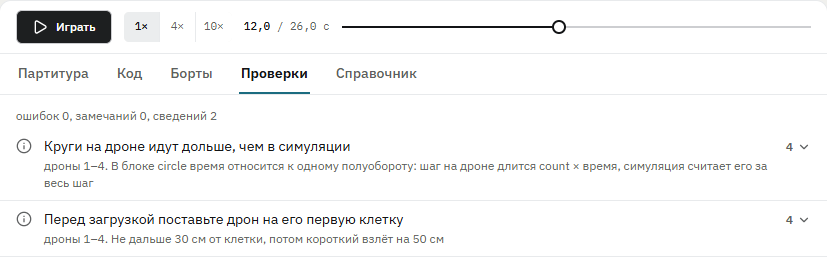
\includegraphics[width=\dimexpr\textwidth-2\fboxrule\relax]{figures/k_checks.png}}
  \caption{Вкладка «Проверки» для шоу «Круг»: два сведения (круги на дроне идут дольше, перед загрузкой поставьте дрон на первую клетку). Ошибок нет. Строку можно раскрыть стрелкой справа.}\label{fig:checks}
\end{figure}

Всего проверяется пять вещей.

\begin{center}
\begin{tabular}{@{}p{3.6cm}p{5.6cm}p{3.6cm}@{}}
\toprule
Что & Правило & Уровень \\
\midrule
Область & дрон не выходит за выбранную область; клетка не больше 143 & ошибка \\
Высота & не выше лимита (по умолчанию 150\cm) & ошибка \\
Скорость & каждый переход не быстрее 100\cm/с & замечание \\
Сближение & дроны не ближе 60\cm друг к другу & замечание \\
Зависание & одно ожидание не длиннее 60\,с & отказ при загрузке \\
\bottomrule
\end{tabular}
\end{center}

Про скорость и сближение вы уже знаете (уроки~\ref{ch:peretyot}, \ref{ch:dva-drona}). Остальное разберём на примерах.

\section{Читаем сообщение}

В каждом сообщении три вещи:
\begin{enumerate}
  \item \textbf{кто}: номер дрона или пара дронов;
  \item \textbf{когда}: время в шоу; передвиньте ползунок на это время и посмотрите;
  \item \textbf{где}: номер строки в коде (щелчок по сообщению показывает её).
\end{enumerate}
Похожие замечания о разных дронах приложение собирает в одну строку, например «Переход быстрее порога… дроны 1--10, быстрейший 120 см/с». Строку можно раскрыть стрелкой.

\section{Три проблемы сразу}

В этом файле нарочно собрано сразу три проблемы:

\solfile{bad_examples/bad_three.py}

Проверка скажет:
\begin{itemize}
  \item ошибка: «Дрон 1: высота 170 см больше лимита 150 см, полёт будет отклонён» (и то же про дрон 2);
  \item замечание: «Дрон 1: переход на клетку 16 за 1 с (120 см, 120 см/с) быстрее порога 100 см/с…»;
  \item замечание: «Дроны 1 и 2 сближаются до 0 см на 11,6 с (порог 60 см)».
\end{itemize}
Чтобы все три исчезли, нужно: понизить высоты, добавить времени переходу и развести дронов по высоте.

\section{Лимит высоты и область}

\textbf{Лимит.} В меню \knopka{Шоу…} над сценой есть раздел «Высота» с полем \knopka{Лимит высоты, см}: оно принимает целые числа от 20 до 200. После смены нажмите \knopka{Проверить} ещё раз. Больше 200 нельзя.

\textbf{Область.} Выбор \knopka{Область} над сценой задаёт рамку (весь коврик или четверть). Если дрон вылетает за неё, будет ошибка «полёт выходит за рабочую область». Тогда смените область, перенесите шоу (меню \knopka{Шоу…}) или поправьте клетки. Сам код выбор области не меняет.

\textbf{Зависание.} Если ожидание на месте длиннее 60 секунд, приложение откажет при \knopka{Загрузить}: «Зависание 90 с больше лимита 60 с». Разбейте ожидание на несколько шагов.

\begin{probuy}
  \item Исправьте все три проблемы файла \texttt{bad\_three.py}, чтобы проверка прошла без замечаний.
  \item В файле \texttt{bad\_height.py} (урок~\ref{ch:vzlet}) высота 180\cm. Не меняя файл, сделайте так, чтобы проверка прошла. Что для этого нужно?
  \item В файле \texttt{bad\_hover.py} дрон висит 90 секунд на одном месте. Исправьте его.
  \item В файле \texttt{bad\_area.py} дрон летит в клетку 8, а выбрана четверть 1. Исправьте файл.
\end{probuy}
\solfile{bad_examples/bad_hover.py}
\solfile{bad_examples/bad_area.py}
\otvety{11}
